\documentclass{beamer}
\usepackage[utf8]{inputenc}
\usepackage{palatino}
\usepackage{subfig}
\usepackage{amsmath}
\usepackage{dsfont}
\usepackage{minted}
\usepackage{multimedia}

\usetheme{Warsaw}
\usecolortheme{crane}

% www.sharelatex.com/learn/Beamer

\title{Probability Distributions}
\author{Brendon J. Brewer}
\institute{Department of Statistics\\
The University of Auckland}
\date{{\tt \color{blue} https://www.stat.auckland.ac.nz/\~{ }brewer/}}

\begin{document}

\frame{\titlepage}


% New slide
\begin{frame}
\frametitle{Probability Distributions}
Suppose a quantity $X$ might be 1, 2, 3, 4, or 5, and we assign probabilities of
$\frac{1}{5}$ to each of those possible values. There is some terminology:

\begin{itemize}
  \item<2-> $X$ is called a `random variable' (not often by me)
  \item<3-> $\{1, 2, 3, 4, 5\}$ is called the `sample space', `hypothesis space',
        or `parameter space'
  \item<4-> $\boldsymbol{p} = \left\{\frac{1}{5}, \frac{1}{5}, \frac{1}{5},
                \frac{1}{5}, \frac{1}{5}\right\}$
        is the `probability distribution' for
        $x$. In this case, it is a {\em discrete uniform} distribution.
\end{itemize}

\visible<5>{
The probability distribution is often written as $P(X=x) =$ (some function of $x$).}

\end{frame}



% New slide
\begin{frame}
\frametitle{Properties of discrete probability distributions}

\pause
Normalisation:\\ $\sum_x P(X=x) = 1$.\vspace{0.5em}

\pause
Expected value:\\$\mathds{E}(X) = \left<X\right> = \sum_x x P(X=x)$\vspace{0.5em}

\pause
Variance:\\$\textnormal{Var}(X) = \mathds{E}\left((X - \mathds{E}(X))^2\right) = \sum_x (x - \mathds{E}(X))^2 P(X=x)$\vspace{0.5em}

\pause
Standard deviation:\\$\textnormal{sd}(X) = \sqrt{\textnormal{Var}(X)}$

\pause
The expected value and sd describe the {\em center} and {\em width}
of the distribution respectively.

\end{frame}


% New slide
\begin{frame}
\frametitle{Shorthand notation}
$P(X=x)$ is cumbersome. $x$ is also just a dummy variable.

Common shorthand notation: 
Use $p(x)$ instead, equivocate between the quantity itself and the dummy
variable. E.g.:
\begin{align}
\mathds{E}(x) = \sum x p(x)
\end{align}

\end{frame}


% New slide
\begin{frame}[t, fragile]
\frametitle{Numerical handling}
Numerical handling of discrete probability distributions for a single
quantity: \vspace{2em}

\begin{minted}{python}
xs = np.arange(5, 21) # Grid of possibilities
ps = xs**2            # Not normalised
ps = ps/ps.sum()      # Normalise it
plt.bar(xs, ps)       # Plot it

# Expected value and variance
ex = np.sum(xs*ps) 
variance = np.sum(ps*(xs - ex)**2)
np.sum(ps[xs >= 10]) # P(x >= 10)
\end{minted}


\end{frame}




% New slide
\begin{frame}[t, fragile]
\frametitle{Common discrete distributions}

Here are some common discrete distributions:

\begin{itemize}
\item <2-> Discrete Uniform (which one is it?)
\item <3-> Binomial (how many successes out of $N$ quasi-identical trials?)
\item <4-> Poisson (how many occurrences of rare event?)
\end{itemize}

\end{frame}


% New slide
\begin{frame}[t, fragile]
\frametitle{Astronomy uses for Discrete Uniform}



\end{frame}


% New slide
\begin{frame}[t, fragile]
\frametitle{Astronomy uses for Binomial}


\end{frame}



% New slide
\begin{frame}[t, fragile]
\frametitle{Astronomy uses for Poisson}


The intensity of an X-ray source is such that you would expect to detect
$\lambda$ photons per minute. Let $x$ be the actual number of photons you
observe in a minute.

\begin{align}
x | \lambda &\sim \textnormal{Poisson}(\lambda) \\
p(x | \lambda) &= \frac{\lambda^x e^{-\lambda}}{x!}
\end{align}

where $\lambda \geq 0$ and $x \in \{0, 1, 2, 3, ..., \}$.


\end{frame}


% New slide
\begin{frame}[t, fragile]
\frametitle{Three Poisson Distributions}

\begin{center}
  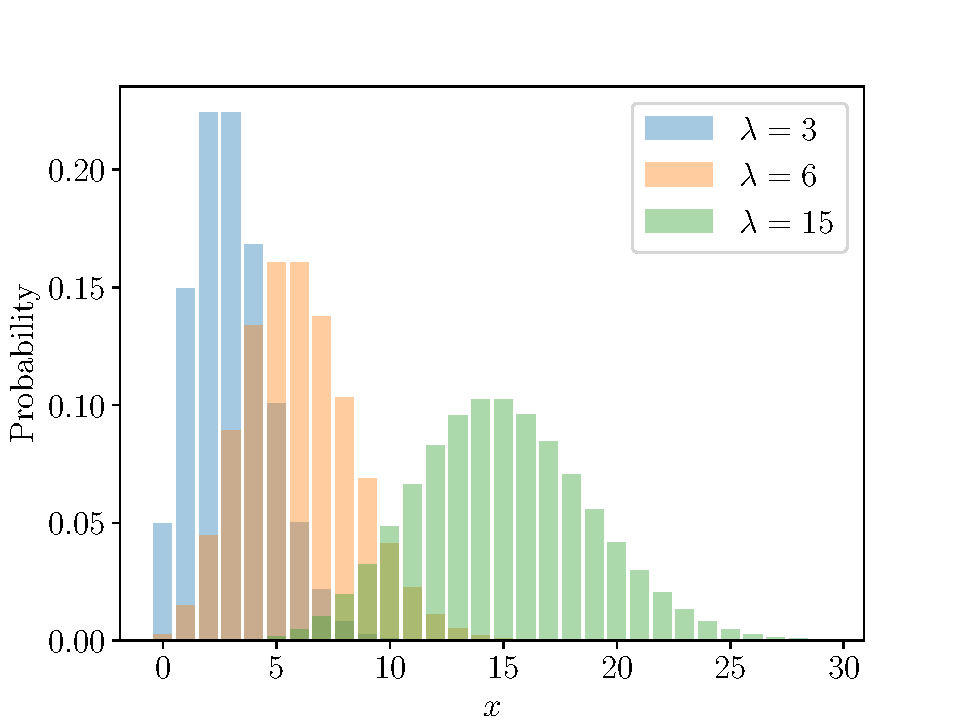
\includegraphics[width=0.7\textwidth]{poisson.pdf}
\end{center}

\end{frame}


% New slide
\begin{frame}[t, fragile]
\frametitle{Continuous distributions}

These are characterised by a continuous hypothesis space (e.g.
``all real numbers'') and a {\em probability density function} (PDF).
\vspace{1em}

For example, normal/gaussian distributions:

\begin{align}
X | \mu, \sigma &\sim \textnormal{Normal}(\mu, \sigma^2) \\
f_X(x) &= \frac{1}{\sigma \sqrt{2\pi}} \exp\left[-\frac{1}{2\sigma^2(x-\mu)^2}\right]
\end{align}


$f_X(x)$ is the full notation favoured by many statisticians.
You can also just write $f(x)$ or $p(x)$ (and not having any upper-case $X$).

\end{frame}


% New slide
\begin{frame}
\frametitle{Properties of continuous probability distributions}

Just like discrete, with integrals (implicitly over all $x$) replacing sums!

\pause
Normalisation:\\ $\int p(x) \, dx = 1$.\vspace{0.5em}

\pause
Expected value:\\$\mathds{E}(X) = \left<X\right> = \int x p(x) \, dx$\vspace{0.5em}

\pause
Variance:\\$\textnormal{Var}(X) = \mathds{E}\left((X - \mathds{E}(X))^2\right) = \int (x - \mathds{E}(X))^2 f(x) \, dx$\vspace{0.5em}

\pause
Standard deviation:\\$\textnormal{sd}(X) = \sqrt{\textnormal{Var}(X)}$

\pause
The expected value and sd describe the {\em center} and {\em width}
of the distribution respectively.

\end{frame}


\end{document}


